\documentclass[10pt]{article}

\usepackage{mathtools}
\DeclarePairedDelimiter\ceil{\lceil}{\rceil}
\DeclarePairedDelimiter\floor{\lfloor}{\rfloor}

\usepackage{algpseudocode}
\usepackage{graphicx}
\graphicspath{{img/}}
\usepackage{amsmath}
\usepackage[margin=1.0in]{geometry}
\usepackage{hyperref}
\hypersetup{
	colorlinks=true,
	linkcolor=blue
}


\begin{document}

\title{\vspace{-2.0cm}Project 3A}
\author{Taylor Nelms and Nikhil Shenoy}
\date{\today}

\maketitle

\section{How to Run}
You can run this project by executing ``python mymosaic.py'' from the command line. The script expects that the images being used for the mosaicing are in a directory one level higher than ``mymosaic.py'' and in a directory called ``test\_img''. If you are in the same directory as ``mymosaic.py'', then the relative path would be ``../test\_img/1L.png''. Place three images in that ``test\_img'' directory. To do a nearest neighbors calculation, we used the KDTree from scipy.spatial.

\section{Image Outputs}

	%% NEED THE COLOR MAP FOR THE CORNER STRENGTH MAP
	\begin{figure}[h]
		\caption{corner map}
		\centering
		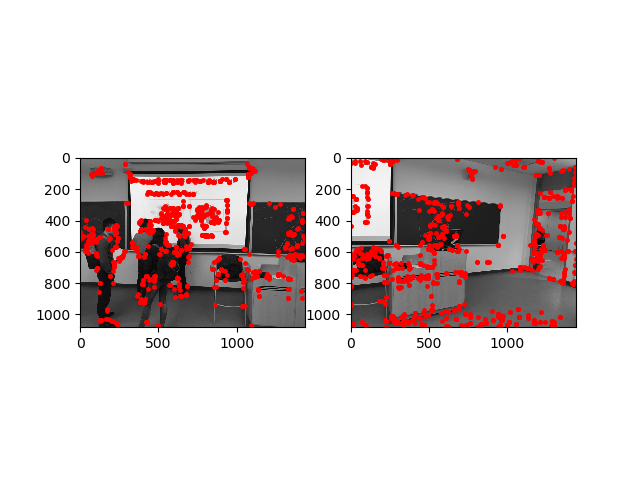
\includegraphics{ANMSl2m.png}
	\end{figure}

	\begin{figure}[h]
		\caption{ANMS for the left image}
		\centering
		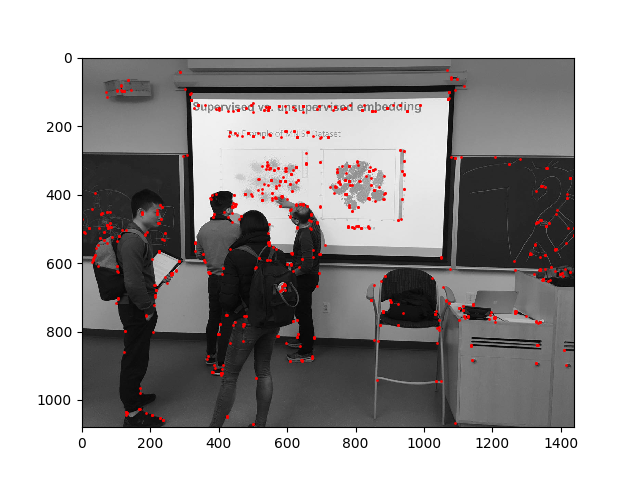
\includegraphics{anmsL.png}
	\end{figure}
	
	\begin{figure}[h]
		\caption{ANMS for the middle image}
		\centering
		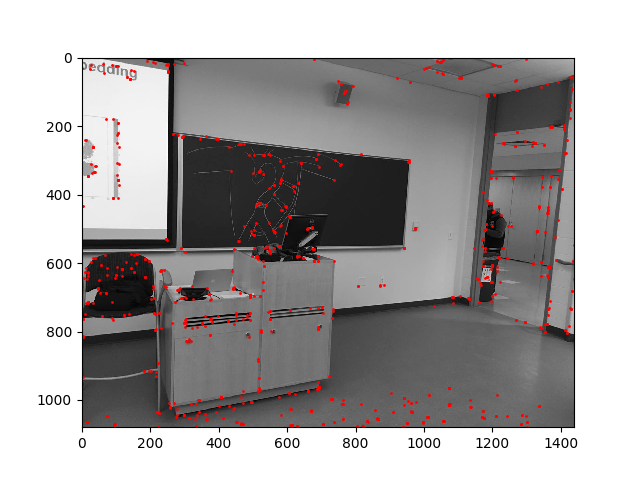
\includegraphics{anmsM.png}
	\end{figure}

    	\begin{figure}[h]
		\caption{ANMS for the right image}
		\centering
		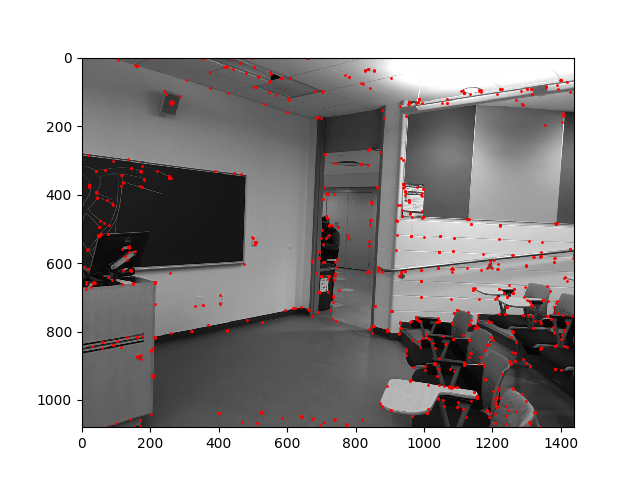
\includegraphics{anmsR.png}
	\end{figure}
        
	\begin{figure}[h]
		\caption{Post-RANSAC points using the left and middle images}
		\centering
		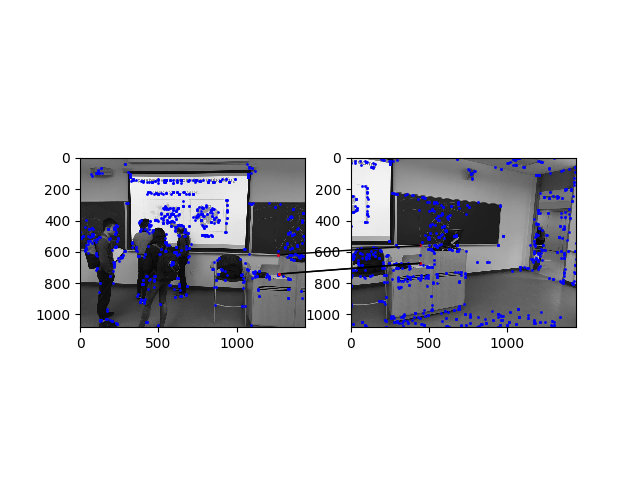
\includegraphics{postranLM.png}
	\end{figure}
	
	\begin{figure}[h]
		\caption{Post-RANSAC points using the middle and right images}
		\centering
		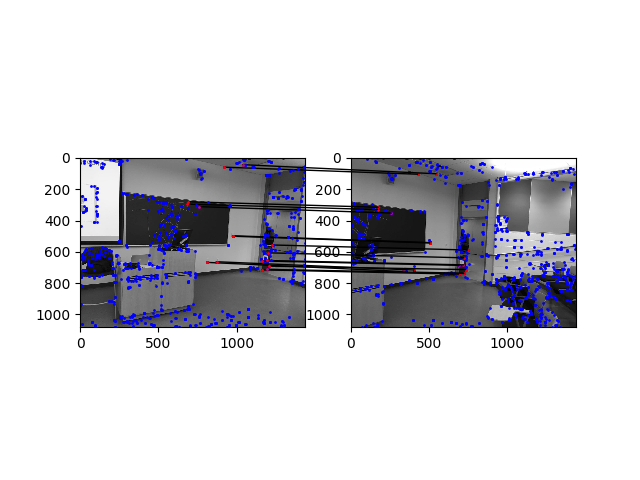
\includegraphics{postranMR.png}
	\end{figure}
	

	\begin{figure}[h]
		\caption{Final panorama}
		\centering
		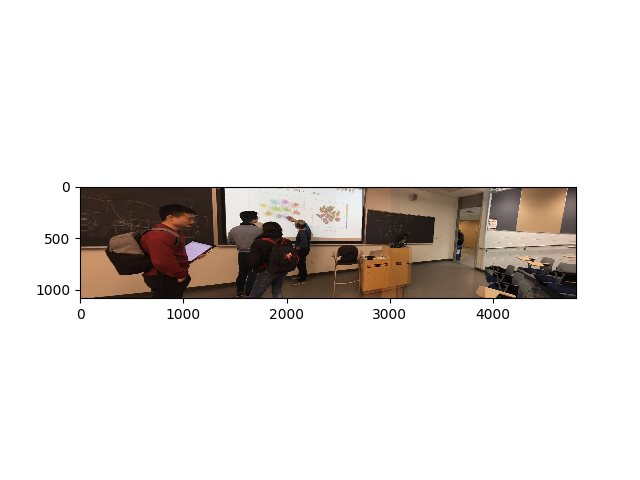
\includegraphics{mosaic.png}
	\end{figure}
\end{document}


